\section{Auswertung}

Untersucht wurden die Ausgangsspannungen am Lock-In-Verstäker in Abhängigkeit von dem Phasenunterschied zwischen Signal- und Referenzspannung. Im Folgenden ist die Auswertung 
für eine Signalspannung mit und ohne Rauschen unterteilt.

\subsection{Ausgangsspannung ohne Rauschen}
In diesem Versuchsteil wurden die Ausgangsspannungen am Lock-In-Verstäker einer mit einer Rechteckspannung modifizierten sinusförmigen Signalspannung gemessen. In der Tabelle ..
sind die Ausgangsspannung $U_{\text{out}}$ in Abhängigkeit von der Phase notiert. An einem Oszilloskop ließen sich Momentanaufnahmen von unverstärkten Signalspannung (in Gelb), sowie den Ausgangsspannungen in Türkis anfertigen.
Die Abbildungen \ref{fig:11} bis \ref{fig:18} zeigen die Spannungen in Abhängigkeit von der Phase $\phi$ welche von $\SI{0}{\degree}$ bis $\SI{360}{\degree}$ verändert werden.
\\
\newline 
Die Beziehung \eqref{eqn:yesss} lässt sich anhand dieser Messwerte mit einer Fitfunktion dieser Art 
\begin{equation}
    \label{eqn:fit}
U_{\text{out}} = a \cdot \text{cos}(b \cdot \frac{180}{\pi} \phi + c) + d,
\end{equation}
überprüfen. Dazu wird ein \enquote{Curvefit} mit \cite{scipy} verwendet.
Es ergeben sich die folgenden Parameter
\begin{align}
    a &= \SI{1}{\volt},\\
    b &= \SI{1}{},\\
    c &= \SI{1}{\radian},\\
    d &= \SI{1}{\volt}.\\
\end{align}
Die Fitfunktion mit diesen Parametern, sowie die einzelnen Messwerte aus Tabelle ... sind in der Abbildung \ref{fig:licht} dargestellt.
\begin{figure}
    \centering
    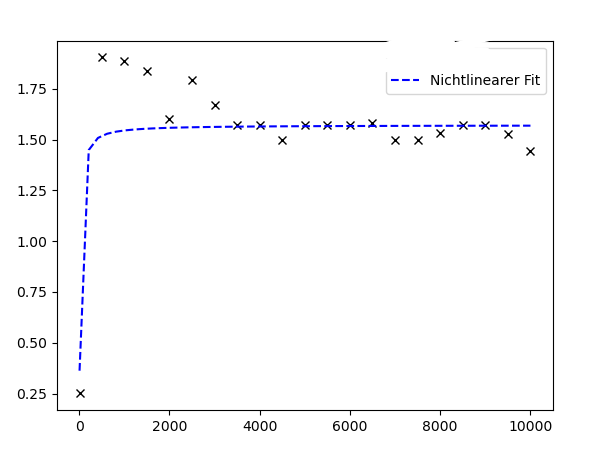
\includegraphics[width=0.9\textwidth]{build/plot1.pdf}
    \caption{Phasenabhängige Ausgangsspannungen ohne Rauschen mit Fitfunktion.} 
    \label{fig:licht}
\end{figure}
\begin{figure}
    \begin{minipage}{0.5\textwidth}
        \centering
        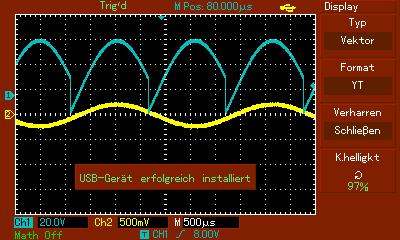
\includegraphics[width=0.8\textwidth]{bilder/0ohne.png}
        \caption{$\phi = \SI{0}{\degree}$.} 
        \label{fig:11}
    \end{minipage}
    \hfill
    \begin{minipage}{0.5\textwidth}
        \centering
        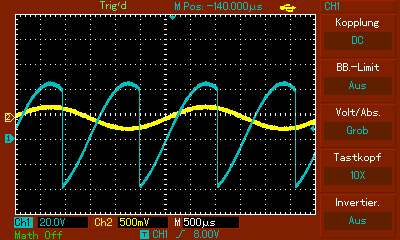
\includegraphics[width=0.8\textwidth]{bilder/45ohne.png}
        \caption{$\phi = \SI{45}{\degree}$.} 
        \label{fig:12}
    \end{minipage}
    \vspace{1cm}
    \vfill
    \begin{minipage}{0.5\textwidth}
        \centering
        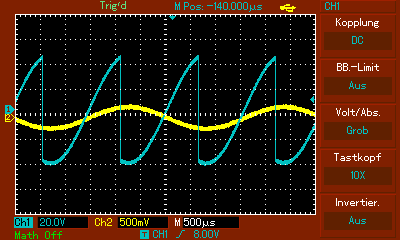
\includegraphics[width=0.8\textwidth]{bilder/90ohne.png}
        \caption{$\phi = \SI{90}{\degree}$.} 
        \label{fig:13}
    \end{minipage}
    \hfill
    \begin{minipage}{0.5\textwidth}
        \centering
        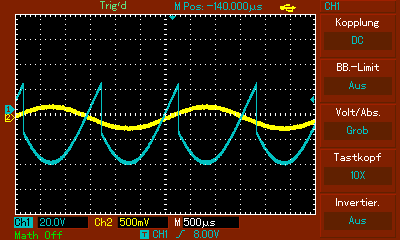
\includegraphics[width=0.8\textwidth]{bilder/135ohne.png}
        \caption{$\phi = \SI{135}{\degree}$.} 
        \label{fig:14}
    \end{minipage}
    \vspace{1cm}
    \vfill
    \begin{minipage}{0.5\textwidth}
        \centering
        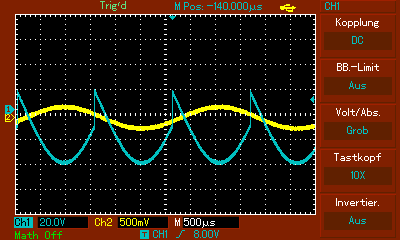
\includegraphics[width=0.8\textwidth]{bilder/180ohne.png}
        \caption{$\phi = \SI{180}{\degree}$.} 
        \label{fig:15}
    \end{minipage}
    \hfill
    \begin{minipage}{0.5\textwidth}
        \centering
        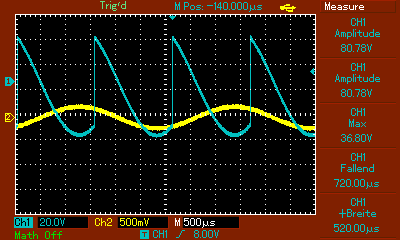
\includegraphics[width=0.8\textwidth]{bilder/240ohne.png}
        \caption{$\phi = \SI{240}{\degree}$.} 
        \label{fig:16}
    \end{minipage}
    \vspace{1cm}
    \vfill
    \begin{minipage}{0.5\textwidth}
        \centering
        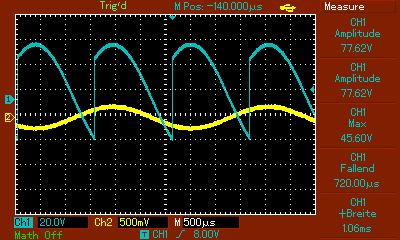
\includegraphics[width=0.8\textwidth]{bilder/300ohne.png}
        \caption{$\phi = \SI{300}{\degree}$.} 
        \label{fig:17}
    \end{minipage}
    \hfill
    \begin{minipage}{0.5\textwidth}
        \centering
        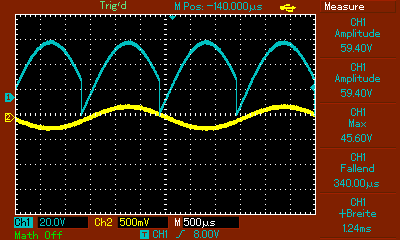
\includegraphics[width=0.8\textwidth]{bilder/360ohne.png}
        \caption{$\phi = \SI{360}{\degree}$.} 
        \label{fig:18}
    \end{minipage}
    \caption{Momentaufnahmen der phasenabhängigen Ausgangspannungen an einem Lock-In-Verstärker ohne Rauschen.}
\end{figure}

\subsection{Ausgangsspannung mit Rauschen}
Die Abbildungen \ref{fig:21} bis \ref{fig:27} zeigen die Ausgangsspannungen in Abhängigkeit von der Phase $\phi$, im Fall der verrauschten Signalspannung.
\\
\newline 
Für diese Auswertung wird das gleiche Verfahren wie ohne Rauschen mit der Messreihe aus Tabelle .. wiederholt. Mit der Beziehung \eqref{eqn:fit} ergeben sich nun die folgenden
Parameter
\begin{align}
    a &= \SI{1}{\volt},\\
    b &= \SI{1}{},\\
    c &= \SI{1}{\radian},\\
    d &= \SI{1}{\volt}.\\
\end{align}
In der Abbildung \ref{tab:licht2} sind nun die Messwerte dieser Messreihe, sowie die Fitfunktion dargestellt.
\begin{figure}
    \centering
    \includegraphics[width=0.6\textwidth]{build/plot2.pdf}
    \caption{Schematischer Aufbau des Lock-In-Verstäker mit installiertem Photodetektor. \cite{skript}} 
    \label{fig:licht2}
\end{figure}
\begin{figure}
    \begin{minipage}{0.5\textwidth}
        \centering
        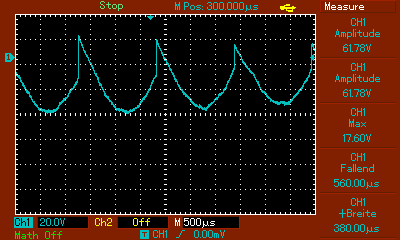
\includegraphics[width=0.8\textwidth]{bilder/0mit.png}
        \caption{$\phi = \SI{0}{\degree}$.} 
        \label{fig:21}
    \end{minipage}
    \hfill
    \begin{minipage}{0.5\textwidth}
        \centering
        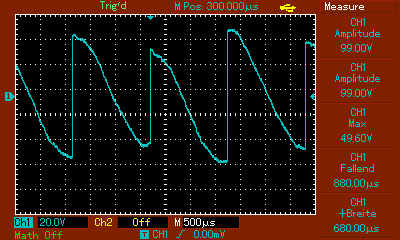
\includegraphics[width=0.8\textwidth]{bilder/60mit.png}
        \caption{$\phi = \SI{60}{\degree}$.} 
        \label{fig:22}
    \end{minipage}
    \vspace{1cm}
    \vfill
    \begin{minipage}{0.5\textwidth}
        \centering
        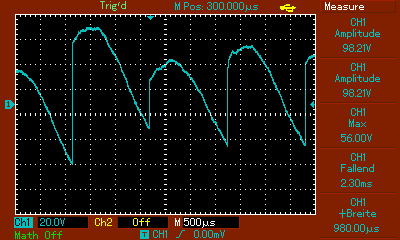
\includegraphics[width=0.8\textwidth]{bilder/120mit.png}
        \caption{$\phi = \SI{120}{\degree}$.} 
        \label{fig:23}
    \end{minipage}
    \hfill
    \begin{minipage}{0.5\textwidth}
        \centering
        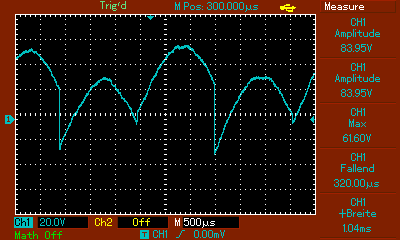
\includegraphics[width=0.8\textwidth]{bilder/180mit.png}
        \caption{$\phi = \SI{180}{\degree}$.} 
        \label{fig:24}
    \end{minipage}
    \vspace{1cm}
    \vfill
    \begin{minipage}{0.5\textwidth}
        \centering
        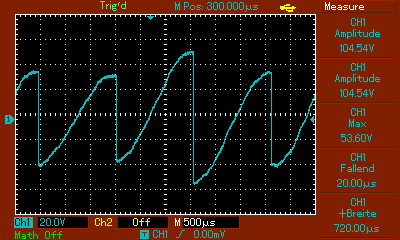
\includegraphics[width=0.8\textwidth]{bilder/240mit.png}
        \caption{$\phi = \SI{240}{\degree}$.} 
        \label{fig:25}
    \end{minipage}
    \hfill
    \begin{minipage}{0.5\textwidth}
        \centering
        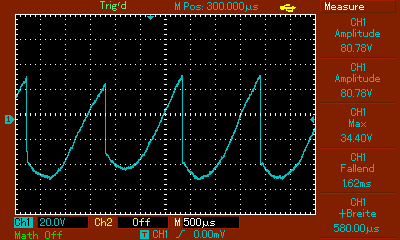
\includegraphics[width=0.8\textwidth]{bilder/300mit.png}
        \caption{$\phi = \SI{300}{\degree}$.} 
        \label{fig:26}
    \end{minipage}
    \vspace{1cm}
    \vfill
        \centering
        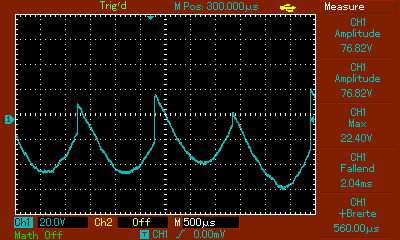
\includegraphics[width=0.4\textwidth]{bilder/360mit.png}
        \caption{$\phi = \SI{360}{\degree}$.} 
        \label{fig:27}
    \caption{Momentaufnahmen der phasenabhängigen Ausgangspannungen an einem Lock-In-Verstärker mit Rauschen.}
\end{figure}